\documentclass[main.tex]{subfiles}
\begin{document}
\newpage
\section{Anhang}

\begin{figure}[H]
    \centering
    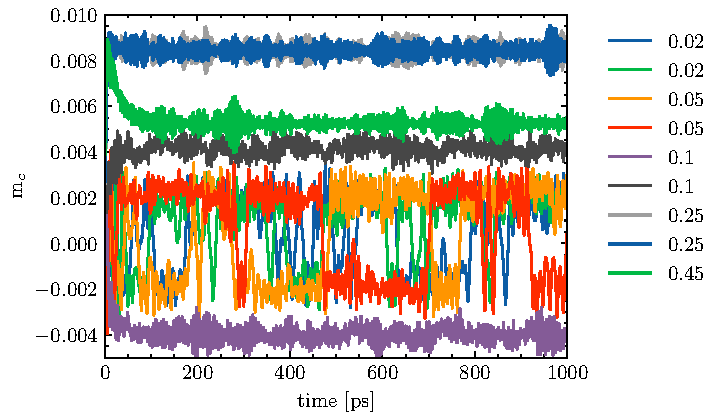
\includegraphics{bilder/plots/dh_variation/mc_time.pdf}
    \caption{Einfluss von Variation der numerischen Schrittweite  auf Rauschsignal \todo{plot hübsch machen und vllt nur eine linie pro h}}\label{fig:dh-variation}
\end{figure}

% \begin{figure}[H]
%     \centering
%     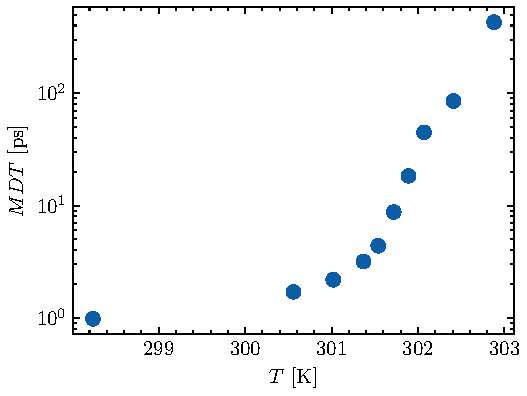
\includegraphics{bilder/plots/temp_comparison_long/mean_dwell_time.pdf}
%     \caption{temp mean dwell time long\todo{auch mdt aus autocorr?} }\label{fig:temp-mdt-long}
% \end{figure}

% \begin{figure}[H]
%     \centering
%     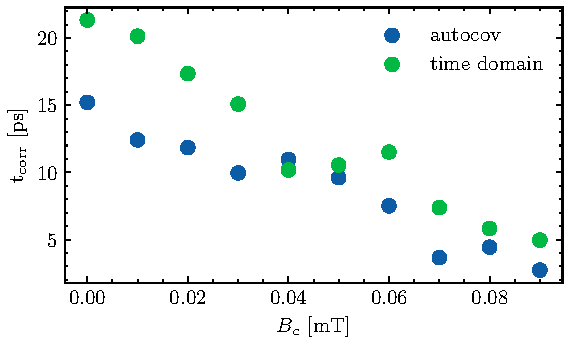
\includegraphics{bilder/plots/max_Bz/t_corr.pdf}
%     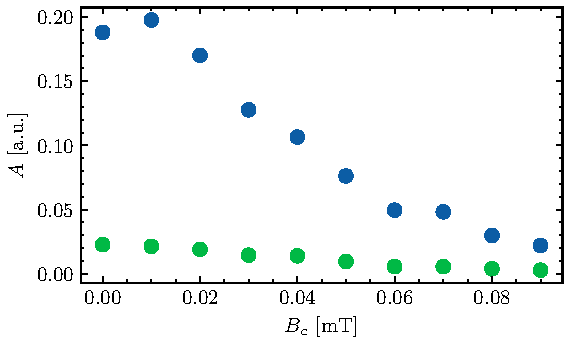
\includegraphics{bilder/plots/max_Bz/amplitude_corr.pdf}
%     \caption{Aus irgendwelchen gründen stimmen Die Datenpunkte nicht miteinander überein \todo{Nachvollziehen, woher die Datenpunkte kommen}\todo{versuchen nochmal neu zu implementieren}\todo{plots überhaupt einbinden?}}\label{fig:bz-autocorr-amplitude}
% \end{figure}


\end{document}